% ME 144L Dynamic Systems & Controls Lab — Comprehensive Study Guide (Labs 1–10)
\documentclass[9pt,twocolumn]{article}

\usepackage[top=0.5in, bottom=0.5in, left=0.45in, right=0.45in]{geometry}
\usepackage{amsmath,amssymb}
\usepackage{booktabs,array,tabularx}
\usepackage[table]{xcolor}
\usepackage{tikz}
\usetikzlibrary{arrows.meta, positioning, calc}
\usepackage{fancybox}
\usepackage{float}
\usepackage[colorlinks=true, allcolors=blue]{hyperref}

\definecolor{accent}{HTML}{BF5700}
\definecolor{bodytext}{HTML}{333333}
\definecolor{ansbg}{HTML}{FFF8F0}
\definecolor{ansframe}{HTML}{D9A87C}
\definecolor{secbg}{HTML}{F5EDE4}

\color{bodytext}
\pagestyle{empty}
\setlength{\parindent}{0pt}
\setlength{\parskip}{2pt}
\setlength{\columnsep}{12pt}
\setlength{\jot}{2pt}

% compact lists
\setlength{\leftmargini}{1.2em}
\setlength{\itemsep}{0pt}
\setlength{\parsep}{0pt}
\setlength{\topsep}{1pt}

% --- Custom commands ---
\newcommand{\labsec}[1]{%
  \vspace{5pt}%
  \noindent\colorbox{accent}{\parbox{\dimexpr\columnwidth-2\fboxsep}{%
    \centering\bfseries\color{white}\small #1}}%
  \vspace{3pt}\par%
}
\newcommand{\subsec}[1]{%
  \vspace{3pt}%
  {\small\bfseries\textcolor{accent}{#1}}%
  \vspace{1pt}\par\noindent%
}
\newcommand{\eqbox}[1]{%
  \par\noindent\centerline{\fboxsep=3pt\fcolorbox{ansframe}{ansbg}{\parbox{0.92\columnwidth}{\small #1}}}%
  \vspace{2pt}\par%
}
\newcommand{\minibox}[1]{%
  \fboxsep=2pt\fcolorbox{ansframe}{ansbg}{\small\textbf{#1}}%
}

\begin{document}
\small
\setlength{\abovedisplayskip}{2pt}
\setlength{\belowdisplayskip}{2pt}
\setlength{\abovedisplayshortskip}{1pt}
\setlength{\belowdisplayshortskip}{1pt}

\begin{center}
{\Large\bfseries\textcolor{accent}{ME 144L --- Study Guide}}\\[2pt]
{\normalsize Labs 1--10 $\mid$ Spring 2026 $\mid$ Alejandro Diaz}
\end{center}
\vspace{2pt}
\hrule height 0.8pt
\vspace{4pt}

% ══════════════════════════════════════════════════════════════
\labsec{Lab 1 --- Inverted Pendulum (Phone Falling)}
% ══════════════════════════════════════════════════════════════

\subsec{Physical Model}
A phone resting on a table edge is modeled as an inverted pendulum pivoting at the table corner. The phone (mass $m$, length $L$) has its center of mass at $L_c = L/2$ from the pivot.

\eqbox{%
Moment of inertia about pivot:\\[2pt]
$J_O = J_{cm} + m L_c^2 = \dfrac{mL^2}{12} + m\!\left(\dfrac{L}{2}\right)^{\!2} = \dfrac{mL^2}{3}$\\[4pt]
Equivalently: \quad $J_O = 2\,m\,L_c^2$
}

\subsec{Equation of Motion}
\[
  J_O\,\dot{\omega} = m\,g\,L_c\,\sin\theta
\]
State--space form with $x = [\theta,\;\omega]^T$:
\[
  \dot{\theta} = \omega, \qquad \dot{\omega} = \frac{m\,g\,L_c}{J_O}\sin\theta
\]

\subsec{Energy Conservation (Peak Speed)}
At release from $\theta=0$ (horizontal), all potential energy converts to rotational kinetic energy at $\theta = \pi/2$:
\eqbox{%
$m\,g\,L_c = \tfrac{1}{2}J_O\,\omega_{\max}^2$\\[3pt]
$\omega_{\max} = \sqrt{\dfrac{2\,m\,g\,L_c}{J_O}} = \sqrt{\dfrac{g}{L_c}} = \sqrt{\dfrac{2g}{L}}$
}

Lab result: $\omega_{\max}^{\text{sim}} = 11.60~\text{rad/s}$, $\omega_{\max}^{\text{exp}} = 12.64~\text{rad/s}$ ($8.6\%$ diff). Gyroscope data from Phyphox app.

\subsec{RK4 Integration}
Used to numerically solve the ODE (see cross-cutting section).

% ══════════════════════════════════════════════════════════════
\labsec{Lab 2 --- Signal Processing \& Flywheel Decay}
% ══════════════════════════════════════════════════════════════

\subsec{RC Low-Pass Filter}
Continuous transfer function:
\[
  H(s) = \frac{1}{\tau s + 1}, \quad \tau = RC, \quad f_c = \frac{1}{2\pi\,\tau}
\]

Cutoff frequency: signals above $f_c$ are attenuated.

\subsec{ZOH Discretization}
Convert continuous filter to discrete-time difference equation via zero-order hold:
\eqbox{%
$y[k] = -a_1\,y[k{-}1] + b_0\,u[k] + b_1\,u[k{-}1]$\\[2pt]
Coefficients from \texttt{scipy.signal.cont2discrete(..., method='zoh')}
}

\subsec{FFT / Spectral Analysis}
Frequency content of a signal is obtained via \texttt{np.fft.fft()}. The FFT shows which frequencies dominate the data --- useful for identifying oscillation frequencies and verifying filter cutoffs.

\subsec{Flywheel Exponential Decay}
First-order spin-down model:
\eqbox{%
$J\,\dot{\omega} = -B\,\omega \;\;\Rightarrow\;\; \omega(t) = \omega_0\,e^{-t/\tau_J}$\\[3pt]
Time constant: $\tau_J = J/B$\\[2pt]
Damping coefficient: $B = J/\tau_J$
}

$\tau_J$ found from level-crossing detection at $V = 0.37\,V_0$ ($= e^{-1}$ of initial). Three cases tested with different damping configurations.

% ══════════════════════════════════════════════════════════════
\labsec{Lab 3 --- Arduino DAQ \& Analog Sensors}
% ══════════════════════════════════════════════════════════════

\subsec{Arduino UNO Specs}
\begin{itemize}
  \item Microcontroller: ATmega328P, 5\,V logic
  \item ADC: 10-bit, range $0$--$5$\,V
  \item Resolution: $5\,\text{V}/1023 \approx 4.9~\text{mV/count}$
  \item 6 analog input pins (A0--A5)
\end{itemize}

\subsec{Potentiometer as Voltage Divider}
Wiper voltage: $V_{\text{out}} = V_s \cdot \dfrac{R_2}{R_1 + R_2}$

As the pot rotates, $R_2/R_\text{total}$ changes linearly, producing a voltage proportional to angle.

\subsec{LED Power}
\eqbox{%
$P = \dfrac{V^2}{R}$\\[2pt]
Example: $P = (5\,\text{V})^2 / 10\,\text{k}\Omega = 2.5~\text{mW}$
}

% ══════════════════════════════════════════════════════════════
\labsec{Lab 4 --- Compound Pendulum Modeling}
% ══════════════════════════════════════════════════════════════

\subsec{Potentiometer Calibration}
Linear sensor model:
\eqbox{%
$\theta\,[\text{deg}] = K \cdot V + \theta_0$\\[2pt]
Lab 4: $K = 45.27~\text{deg/V}$, $\theta_0 = -108.5~\text{deg}$, $R^2 = 0.995$
}

\subsec{Equation of Motion}
\eqbox{%
$J_O\,\ddot{\theta} = -m\,g\,L_c\sin\theta \;-\; b\,\dot{\theta} \;-\; \tau_0\,\text{sign}(\dot{\theta})$\\[4pt]
\begin{tabular}{ll}
$J_O$ & Moment of inertia about pivot\\
$L_c$ & Pivot to center of mass\\
$b$ & Viscous damping coeff.\\
$\tau_0$ & Coulomb friction torque\\
\end{tabular}
}

\subsec{Friction Types}
\begin{itemize}
  \item \textbf{Viscous}: $\tau_v = b\,\dot{\theta}$ --- proportional to velocity, continuous
  \item \textbf{Coulomb}: $\tau_c = \tau_0\,\text{sign}(\dot{\theta})$ --- constant magnitude, opposes motion, causes linear amplitude decay
\end{itemize}

In Lab 4, Coulomb friction dominated (${\sim}165\times$ viscous contribution).

\subsec{Small-Angle Natural Frequency}
$\sin\theta \approx \theta$ for small angles:
\[
  \omega_n = \sqrt{\frac{m\,g\,L_c}{J_O}}
\]

\subsec{State--Space Form for RK4}
\[
  \dot{\theta} = \omega, \qquad \dot{\omega} = \frac{1}{J_O}\!\left[-m g L_c\sin\theta - b\omega - \tau_0\,\text{sign}(\omega)\right]
\]

% ══════════════════════════════════════════════════════════════
\labsec{Lab 5 --- IMU \& Cantilever Beam Vibration}
% ══════════════════════════════════════════════════════════════

\subsec{LSM6DSO IMU}
\begin{center}
\small
\begin{tabular}{lcc}
\toprule
 & Accelerometer & Gyroscope\\
\midrule
Range & $\pm 2g$ & $\pm 250~\text{dps}$\\
Sensitivity & $0.061\times10^{-3}~g/\text{LSB}$ & $8.75~\text{mdps/LSB}$\\
\bottomrule
\end{tabular}
\end{center}

\subsec{Acceleration Conversion ($\pm2g$ range)}
\eqbox{%
$a\,[\text{m/s}^2] = z_a \times 2 \times (0.061\times10^{-3}) \times 9.81$\\[2pt]
where $z_a$ is the raw integer count from the sensor.
}

\subsec{Cantilever Beam Stiffness}
\eqbox{%
$k_b = \dfrac{3\,E\,I}{L^3}$, \qquad $I = \dfrac{b\,h^3}{12}$\\[4pt]
$E$ = Young's modulus, $b$ = beam width, $h$ = beam thickness, $L$ = free length
}

\subsec{Effective Mass}
A distributed-mass cantilever does not vibrate like a point mass. The correction:
\eqbox{%
$m_{\text{eff}} = m_{\text{tip}} + 0.23\,m_{\text{beam}}$
}

\subsec{Vibration Analysis Pipeline}
\begin{enumerate}
  \item Record free vibration (IMU accelerometer data)
  \item Find peaks $\to$ get amplitudes $A_n$ and times $t_n$
  \item Damped period: $T_d = \text{mean}(\Delta t_{\text{peaks}})$
  \item Log decrement $\to$ $\beta$, $\zeta$ (see cross-cutting)
  \item $\omega_d = 2\pi/T_d$, \quad $\omega_n = \omega_d/\sqrt{1-\zeta^2}$
  \item Back-calc stiffness: $k = \omega_n^2 \cdot m_{\text{eff}}$
\end{enumerate}

Lab 5 results: $\beta = 0.0093$, $\zeta = 1.4\times10^{-5}$, $\omega_d = 60.75~\text{rad/s}$, $k = 218.80~\text{N/m}$ (at $L = 0.40~\text{m}$).

% ══════════════════════════════════════════════════════════════
\labsec{Lab 6 --- Load Cell \& Bungee Cord Dynamics}
% ══════════════════════════════════════════════════════════════

\subsec{Wheatstone Bridge}
\eqbox{%
$V_{\text{out}} = V_s\!\left(\dfrac{R_3}{R_3+R_4} - \dfrac{R_2}{R_1+R_2}\right)$
}
When all resistors are equal, $V_{\text{out}}=0$. A strain gage in one arm changes resistance under load, unbalancing the bridge to produce $V_{\text{out}} \propto \text{strain}$.

\subsec{Load Cell Calibration}
Linear regression of known masses vs.\ ADC counts:
\eqbox{%
$\text{Mass [g]} = 3.40\times10^{-4}\cdot x - 141.878$, \quad $R^2 = 0.9999$\\[2pt]
Sensitivity: $S = 3.34\times10^{-6}~\text{N/count}$
}

\subsec{Bungee Cord Stiffness}
\begin{itemize}
  \item Static stiffness (slope of $F$ vs.\ $\Delta x$): $k_{\text{static}} = 36.65~\text{N/m}$
  \item Dynamic stiffness (from $\omega_n$): $k_{\text{dyn}} = \omega_n^2 \cdot m = 714.6~\text{N/m}$
  \item Difference: bungee is nonlinear --- dynamic stiffness reflects tangent stiffness near equilibrium, which is much higher than the bulk slope
\end{itemize}

\subsec{Force from Acceleration}
Newton's 2nd law check: $F_{\text{acc}}(t) = -m\,a_z(t)$

Compare load-cell force trace to $-m\,a_z$ from the IMU.

\subsec{Damping Results}
$\beta = 0.0485$, $\zeta = 7.71\times10^{-3}$, $\omega_d = 84.56~\text{rad/s}$ ($13.46~\text{Hz}$). Lightly damped system.

\subsec{Strain-Gage vs.\ Piezoelectric Sensors}
\begin{center}
\small
\begin{tabular}{lcc}
\toprule
 & Strain Gage & Piezoelectric\\
\midrule
Measures & Static + dynamic & Dynamic only\\
Principle & Resistance change & Charge generation\\
Freq.\ range & DC to ${\sim}$kHz & Hz to MHz\\
Drift & Low & High (charge leaks)\\
\bottomrule
\end{tabular}
\end{center}

% ══════════════════════════════════════════════════════════════
\labsec{Lab 7 --- Two-Can Fluid System}
% ══════════════════════════════════════════════════════════════

\subsec{Torricelli Outflow}
Volume-based form:
\eqbox{%
$Q_i = K_i\sqrt{V_i}$\\[2pt]
$K$ has units $[\sqrt{\text{mL}}/\text{s}]$; depends on orifice size and can geometry
}

Pressure-based (from slides): $Q = C_c\,A_o\sqrt{2P/\rho}$

\subsec{Ideal $K$ Derivation}
From the orifice equation:
\[
  K_{\text{ideal}} = A_o\sqrt{\frac{2g}{A_{\text{can}}}}
\]
where $A_o$ = orifice area, $A_{\text{can}}$ = can cross-section.

\subsec{Experimental $K$}
From single-can emptying time $T_e$ starting at volume $V_o$:
\eqbox{%
$K = \dfrac{2\sqrt{V_o}}{T_e}$
}

\subsec{State Equations}
\eqbox{%
$\dot{V}_1 = -K_1\sqrt{V_1}$\\[3pt]
$\dot{V}_2 = K_1\sqrt{V_1} - K_2\sqrt{V_2}$
}

Equilibrium: $\dot{V}_2 = 0 \;\Rightarrow\; K_1\sqrt{V_1^*} = K_2\sqrt{V_2^*}$

\subsec{Hydraulic Capacitance (from slides)}
Tank modeled as a C-element:
\[
  P = \rho\,g\,h = \frac{V}{A\,\rho\,g} \cdot (\rho g)^2 = \frac{V}{C}, \quad C = \frac{A}{\rho\,g}
\]

$C$ relates stored volume to pressure. Larger $A$ $\to$ larger $C$ $\to$ slower draining.

\subsec{Simulation}
Solved with RK4. Two $K$ values tested; plots of $V_1(t)$, $V_2(t)$, $Q_1(t)$, $Q_2(t)$.

% ══════════════════════════════════════════════════════════════
\labsec{Lab 8 --- Computer Vision with OpenCV}
% ══════════════════════════════════════════════════════════════

\subsec{Angle from Three Points}
Given three clicked points (reference, vertex, position), the angle at the vertex:
\eqbox{%
$\vec{v}_1 = P_{\text{ref}} - P_{\text{vertex}}$, \quad $\vec{v}_2 = P_{\text{pos}} - P_{\text{vertex}}$\\[3pt]
$\theta = \arccos\!\left(\dfrac{\vec{v}_1 \cdot \vec{v}_2}{|\vec{v}_1|\,|\vec{v}_2|}\right)$\\[3pt]
Result in $[0^\circ,\;180^\circ]$
}

Expanded:
\[
  \vec{v}_1\cdot\vec{v}_2 = (x_r{-}x_v)(x_p{-}x_v) + (y_r{-}y_v)(y_p{-}y_v)
\]

\subsec{HoughCircles Detection}
\begin{enumerate}
  \item Convert to grayscale
  \item Median blur (kernel size 5)
  \item \texttt{cv2.HoughCircles(gray, HOUGH\_GRADIENT, dp=1, minDist=10, param1=50, param2=40)}
\end{enumerate}

\subsec{Contour-Based Tracking Pipeline}
\begin{enumerate}
  \item Select ROI (\texttt{cv2.selectROI}) on reference frame
  \item Crop each frame to ROI
  \item Convert to grayscale
  \item Binary threshold (inverted for dark dot on light background)
  \item \texttt{cv2.findContours} $\to$ keep largest contour by area
  \item \texttt{cv2.minEnclosingCircle} $\to$ centroid $(x_c, y_c)$
\end{enumerate}

\subsec{Pixel-to-Physical Scale}
\eqbox{%
$\text{scale} = \dfrac{\text{ruler\_length [in]}}{\text{frame\_width [px]}}$\\[3pt]
$x_{\text{real}} = \text{scale}\cdot x_{\text{px}}$, \quad $y_{\text{real}} = \text{scale}\cdot(\text{height} - y_{\text{px}})$
}

$y$ is flipped because image coordinates have $y$ increasing downward.

\subsec{Time-Stamping Methods}
\begin{itemize}
  \item \textbf{Constant FPS}: $t = i/\text{FPS}$ --- assumes constant rate
  \item \textbf{MSEC property}: \texttt{cap.get(cv2.CAP\_PROP\_POS\_MSEC)}
  \item \textbf{\texttt{time()} function}: wall-clock --- most accurate for real-world velocity
  \item \textbf{Frame number}: $t = \text{frame}/\text{FPS}$
\end{itemize}

Frame-based methods overestimate velocity if actual FPS $<$ nominal FPS.

% ══════════════════════════════════════════════════════════════
\labsec{Lab 9 --- PMDC Motor Modeling}
% ══════════════════════════════════════════════════════════════

\subsec{Gyrator Relations (Motor Constant $r_m$)}
\eqbox{%
$\tau_m = r_m\,i_m$ \quad (torque from current)\\[2pt]
$V_m = r_m\,\omega_m$ \quad (back-EMF from speed)\\[3pt]
Power balance: $P_{\text{elec}} = V_m\,i_m = \tau_m\,\omega_m = P_{\text{mech}}$
}

$r_m$ is found as the slope of a linear fit of $V_m$ vs.\ $\omega_m$.

\subsec{Back-EMF Calculation}
\eqbox{%
$V_m = V_{in} - R_m\,i_m$
}
Steady-state assumption: inductive drop $L\,di/dt = 0$.

\subsec{Motor Parameters (Lab 9 Results)}
\begin{center}
\small
\begin{tabular}{lc}
\toprule
$r_m$ (motor constant) & $1.011\times10^{-2}~\text{V\,s/rad}$\\
$R_m$ (armature resistance) & $26.9~\Omega$\\
$B_m$ (viscous damping) & $4.71\times10^{-7}~\text{N\,m\,s/rad}$\\
$\tau_c$ (Coulomb friction) & $9.81\times10^{-5}~\text{N\,m}$\\
$GR$ (gear ratio) & 45\\
$J_m$ (rotor inertia) & $1.45\times10^{-7}~\text{kg\,m}^2$\\
$V_b$ (bus voltage) & $4.82~\text{V}$\\
\bottomrule
\end{tabular}
\end{center}

\subsec{Friction Torque Model}
At no-load steady state, all motor torque is consumed by friction:
\[
  \tau_m = r_m\,i_m = B_m\,\omega_m + \tau_c
\]
$B_m$ = slope and $\tau_c$ = intercept of $\tau_m$ vs.\ $\omega_m$ regression.

\subsec{Torque--Speed Curve (Motor Shaft)}
\eqbox{%
$\tau_o = \dfrac{r_m}{R_m}\,V_{in} - \left(\dfrac{r_m^2}{R_m} + B_m\right)\omega_m$\\[4pt]
Stall torque ($\omega_m=0$): $\tau_s = \dfrac{r_m}{R_m}\,V_{in}$\\[3pt]
No-load speed ($\tau_o=0$): $\omega_{NL} = \dfrac{r_m\,V_{in}}{r_m^2 + R_m\,B_m}$
}

\subsec{Output Shaft (with Gearbox)}
\eqbox{%
$\omega_o = \omega_m / GR$, \quad $\tau_o = GR\cdot\tau_m$\\[4pt]
$\tau_o(\omega_o) = GR\,\dfrac{r_m}{R_m}\,V_{in} - GR^2\!\left(\dfrac{r_m^2}{R_m}+B_m\right)\omega_o$
}

Increasing $V_{in}$ shifts curves upward (parallel lines).

% ══════════════════════════════════════════════════════════════
\labsec{Lab 10 --- PMDC Motor Speed Control}
% ══════════════════════════════════════════════════════════════

\subsec{Open-Loop Control}
Invert the steady-state torque--speed model to find the voltage needed for desired speed $\omega_d$:
\eqbox{%
$V_{in}(\omega_d) = r_m\,\omega_d + \dfrac{R_m}{r_m}\!\left[B_m\,\omega_d + \tau_{c}\tanh(\omega_d)\right]$\\[4pt]
$\text{PWM}(\omega_d) = 255 \cdot \dfrac{V_{in}(\omega_d)}{V_b}$
}

$\tanh(\omega_d)$ is a smooth approximation to $\text{sign}(\omega_d)$ for the Coulomb term.

\subsec{Open-Loop Results}
\begin{center}
\small
\begin{tabular}{cccc}
\toprule
RPM & $\text{PWM}_{\text{exp}}$ & $\text{PWM}_{\text{sim}}$ & $\Delta$PWM\\
\midrule
3250 & 230 & 218.4 & $-5.0\%$\\
2030 & 155 & 141.6 & $-8.6\%$\\
860  & 80  & 68.0  & $-15.1\%$\\
\bottomrule
\end{tabular}
\end{center}
PWM error grows at low speed: model underestimates friction losses.

\subsec{Closed-Loop (Feedback) Control}

\begin{center}
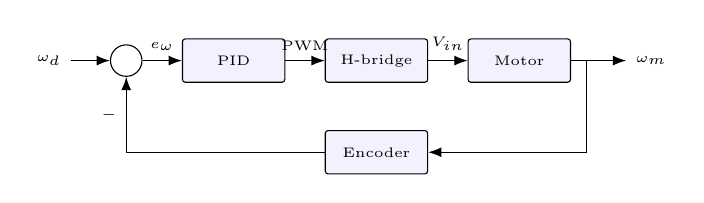
\begin{tikzpicture}[
    node distance=0.9cm and 0.7cm,
    block/.style={draw, rectangle, rounded corners=1pt, minimum width=1.3cm, minimum height=0.55cm, align=center, fill=blue!5, font=\tiny},
    sum/.style={draw, circle, minimum size=0.4cm, inner sep=0pt, font=\tiny},
    >=Latex,
    font=\tiny,
]
    \node (ref)  at (0,0)                       {$\omega_d$};
    \node[sum,   right=0.5cm of ref]     (sum) {};
    \node[block, right=0.5cm of sum]     (ctrl) {PID};
    \node[block, right=0.5cm of ctrl]    (drv)  {H-bridge};
    \node[block, right=0.5cm of drv]     (plant){Motor};
    \node       [right=0.7cm of plant]   (out)  {$\omega_m$};
    \node[block, below=0.6cm of drv]     (enc)  {Encoder};

    \draw[->] (ref)    -- (sum);
    \draw[->] (sum)    -- (ctrl) node[midway, above] {$e_\omega$};
    \draw[->] (ctrl)   -- (drv)  node[midway, above] {PWM};
    \draw[->] (drv)    -- (plant) node[midway, above] {$V_{in}$};
    \draw[->] (plant)  -- (out);
    \draw[->] ($(plant.east)+(0.2,0)$) |- (enc);
    \draw[->] (enc)    -| (sum) node[near end, left] {$-$};
\end{tikzpicture}
\end{center}

Error signal: $e_\omega = \omega_d - \omega_m$

PID controller converts error to PWM command.

\subsec{Advantages of Closing the Loop}
\begin{itemize}
  \item Integral term eliminates steady-state error (compensates model inaccuracy)
  \item Rejects disturbances: voltage drift, load spikes, temperature changes
  \item No need to re-characterize motor when conditions change
  \item Easier to swap motors --- just retune gains
\end{itemize}

\subsec{Disadvantages of Closing the Loop}
\begin{itemize}
  \item Requires working sensor (dead encoder $\to$ no feedback)
  \item Gain tuning ($K_p$, $K_i$, $K_d$, sample rate) requires iteration
  \item Integrator windup: if PWM saturates at $\pm255$, integral accumulates $\to$ overshoot when returning to range
\end{itemize}

% ══════════════════════════════════════════════════════════════
\labsec{Cross-Cutting: 2nd-Order Systems}
% ══════════════════════════════════════════════════════════════

\subsec{Standard Form}
\[
  m\ddot{x} + c\dot{x} + kx = F(t)
\]
Normalized: $\ddot{x} + 2\zeta\omega_n\dot{x} + \omega_n^2 x = F(t)/m$

\eqbox{%
$\omega_n = \sqrt{k/m}$ \quad (undamped natural frequency)\\[2pt]
$\zeta = \dfrac{c}{2\sqrt{k\,m}}$ \quad (damping ratio)\\[2pt]
$\omega_d = \omega_n\sqrt{1-\zeta^2}$ \quad (damped natural frequency)
}

\begin{center}
\small
\begin{tabular}{lcl}
\toprule
Regime & $\zeta$ & Response\\
\midrule
Underdamped & $0 < \zeta < 1$ & Decaying oscillation\\
Critically damped & $\zeta = 1$ & Fastest non-oscillatory\\
Overdamped & $\zeta > 1$ & Slow exponential\\
\bottomrule
\end{tabular}
\end{center}

% ══════════════════════════════════════════════════════════════
\labsec{Cross-Cutting: Log Decrement Method}
% ══════════════════════════════════════════════════════════════

Used in Labs 5 and 6 to extract damping from free-vibration data.

\subsec{Full Pipeline}
\begin{enumerate}
  \item Zero-mean the signal (subtract steady-state tail average)
  \item Detect positive peaks $\to$ amplitudes $A_0, A_1, \ldots, A_n$
  \item Get peak times $\to$ damped period $T_d = \text{mean}(\Delta t)$
  \item Compute $\ln(A_0/A_n)$ for each $n$
  \item Linear regression of $\ln(A_0/A_n)$ vs.\ $n$ $\to$ slope = $\beta$
  \item Damping ratio from $\beta$
  \item Frequencies and stiffness
\end{enumerate}

\eqbox{%
$\ln\!\left(\dfrac{A_0}{A_n}\right) = \beta \cdot n$, \quad where $\beta = \dfrac{2\pi\zeta}{\sqrt{1-\zeta^2}}$\\[6pt]
$\boxed{\;\zeta = \dfrac{\beta}{\sqrt{4\pi^2 + \beta^2}}\;}$ \quad (exact)\\[6pt]
For light damping ($\zeta \ll 1$): $\beta \approx 2\pi\zeta$\\[4pt]
$\omega_d = 2\pi/T_d$, \quad $\omega_n = \omega_d/\sqrt{1-\zeta^2}$, \quad $k = \omega_n^2\,m$
}

% ══════════════════════════════════════════════════════════════
\labsec{Cross-Cutting: RK4 Integrator}
% ══════════════════════════════════════════════════════════════

Fourth-order Runge--Kutta for $\dot{x} = f(x,t)$ with step size $h$:
\eqbox{%
$k_1 = f(x_i,\; t_i)$\\
$k_2 = f(x_i + k_1\,h/2,\; t_i + h/2)$\\
$k_3 = f(x_i + k_2\,h/2,\; t_i + h/2)$\\
$k_4 = f(x_i + k_3\,h,\; t_i + h)$\\[4pt]
$x_{i+1} = x_i + \dfrac{h}{6}(k_1 + 2k_2 + 2k_3 + k_4)$
}

Used for: pendulum (Lab 1, 4), two-can system (Lab 7), motor ODE (Lab 10).

% ══════════════════════════════════════════════════════════════
\labsec{Cross-Cutting: Sensor Calibration}
% ══════════════════════════════════════════════════════════════

General linear model:
\[
  y_{\text{phys}} = K \cdot V_{\text{raw}} + y_0
\]
$K$ = sensitivity (gain), $y_0$ = offset. Found via linear regression of known inputs vs.\ sensor readings.

\begin{center}
\small
\begin{tabular}{lcl}
\toprule
Sensor & $K$ & Units\\
\midrule
Potentiometer (Lab 4) & 45.27 & deg/V\\
Load cell (Lab 6) & $3.40\times10^{-4}$ & g/count\\
Back-EMF (Lab 9) & $1.011\times10^{-2}$ & V$\cdot$s/rad\\
\bottomrule
\end{tabular}
\end{center}

% ══════════════════════════════════════════════════════════════
\labsec{Quick Reference Table}
% ══════════════════════════════════════════════════════════════

\begin{center}
\renewcommand{\arraystretch}{1.3}
\small
\begin{tabular}{p{2.6cm}l}
\toprule
\textbf{Quantity} & \textbf{Formula}\\
\midrule
Log dec.\ slope & $\beta = \text{slope of } \ln(A_0/A_n)$ vs $n$\\
Damping ratio & $\zeta = \beta/\sqrt{4\pi^2+\beta^2}$\\
Damped freq. & $\omega_d = 2\pi/T_d$\\
Undamped freq. & $\omega_n = \omega_d/\sqrt{1-\zeta^2}$\\
Stiffness & $k = \omega_n^2\,m$\\
Pendulum $\omega_n$ & $\sqrt{mgL_c/J_O}$\\
Phone $\omega_{\max}$ & $\sqrt{2gm L_c/J_O}$\\
Beam $k_b$ & $3EI/L^3$\\
Area moment & $I = bh^3/12$\\
Effective mass & $m_{\text{tip}} + 0.23\,m_{\text{beam}}$\\
Torricelli & $Q = K\sqrt{V}$\\
Exp.\ $K$ & $2\sqrt{V_o}/T_e$\\
RC cutoff & $f_c = 1/(2\pi RC)$\\
Flywheel $\tau_J$ & $J/B$\\
ADC resolution & $5\,\text{V}/1023$\\
Motor const. & $r_m = \Delta V_m / \Delta\omega_m$\\
Back-EMF & $V_m = V_{in} - R_m\,i_m$\\
Motor torque & $\tau_m = r_m\,i_m$\\
Torque--speed & $(r_m/R_m)V_{in} - (r_m^2/R_m+B_m)\omega_m$\\
Output $\tau_o$ & $GR\cdot\tau_m$; $\omega_o = \omega_m/GR$\\
OL PWM & $255 \cdot V_{in}/V_b$\\
Scale (vision) & ruler\_len / frame\_width\\
Force--accel & $F = -m\,a_z$\\
\bottomrule
\end{tabular}
\end{center}

\end{document}
